
\section{De Haas-van Alphen torque measurement}

In this section the measurement of \ac{dHvA} oscillations by the torque method is described. For decades, the measurement of \ac{dHvA} oscillations provided the principle method of characterising the Fermiology of a material with only relatively recent competition from techniques such as positron annihilation and \ac{ARPES} in particular. Whilst \ac{ARPES} can provide direct maps of Fermi surfaces within the Brillouin zone, \ac{dHvA} has some advantages such as the fact that it ignores surface effects such as crystal reconstruction, can determine cross-sectional areas with a relatively high resolution and also provides useful secondary measurements such as effective masses of the quasiparticle carriers.  Some disadvantages of the technique include the fact that \ac{dHvA} cannot locate particular cross-sectional orbits within the Brillouin zone (thus relies on secondary knowledge such as \ac{DFT} calculations) and also that the high magnetic fields could potentially affect the Fermi surface, for example by splitting the energy levels. Regardless \ac{dHvA} continues to be a reliable technique for Fermi surface characterisation. A more detailed comparison of all three techniques can be found in appendix~\ref{Appendix:FermilogyTechniques}.

\subsection{Experimental apparatus}

Much of the experiment apparatus has already been described in great detail by Dr. C. Andrew in her thesis\cite{Andrew2010} and so only a broad overview and points of difference will be described here. Moreover, although important experimental parameters will be specified, full details of the configuration of the hardware is listed in appendix~\ref{Appendix:dHvAHardwareSetup}.

\subsubsection{Torque cantilever}

A highly sensitive measure of torque is required to pick up the moments experienced by the sample due to the field. For this reason a commercial piezoelectric \ac{AFM} cantilever, provided by Seiko corps., was repurposed to measure this. The sample was placed onto the topside of the lever above the \ac{AFM} tip. Previously this would be superglued in place but for these measurements we tried successfully with using vacuum grease which freezes the sample in place at low temperatures. This has the added benefit of still being adjustable and removable when warmed back to room temperature. Moreover, when it comes to rotate the sample in the basel plane, this was possible by nudging the sample gently without having to remove the cantilever and risk breaking the lever with the sample permanently affixed.

The cantilevers feature a second dummy lever alongside the principle lever where the sample was mounted. Instead of measuring the voltage across the principle lever alone, we measure the difference of the voltages between the two levers using a Wheatstone bridge. This enables some degree of correction due to vibrations and so on. The circuit can be balanced using a variable resistor and is zeroed as best as possible within the noise before each measurement run.

The voltage is supplied and measured using Stanford SR830 lock-in amplifier. The output is first amplified using an EG\&G 5113 pre-amplifier with a gain of $\times1000$ with a band pass filter which was suitably set for the lock-in amplifier excitation frequency.

\subsubsection{Yellow Magnet}

Measurements of the oscillations were all performed in Bristol on the `Yellow Magnet' system which was built by Oxford and can nominally operate up to \unit[20]{T} with use of the lambda plate, an additional cooling system for the magnet coil, although is more typically operated up to \unit[18]{T}.

The bulk of the cryostat sits in a bath of $^4$He which takes the temperature down to $\approx$\unit[4.2]{K}, and then the sealed sample space is additionally immersed in $^3$He gas in a Heliox system. This system lowers the sample stage temperature to \unit[$\sim0.3$]{K} for several hours before it has to be recondensed. Temperature is monitored at the sample by a Cernox thermometer on the sample stage, and a RuOx thermometer which is mounted in the sample space on the cryostat but is in thermal contact with the tip of the sample stage when the stage is properly inserted into place. Care should be taken that this is the case to ensure good cooling of the sample from the condensed $^3$He. A large mismatch in the temperatures of the Cernox and RuOx thermometers at zero field and base temperature is a good indicator of the sample stage not being seated correctly in the cryostat. Further thermometers are situated on the \unit[1]{K} pot, the sorb and sat on top of the magnet coil although this is only monitored when initially cooling the magnet from room temperature. All thermometers and heaters were controlled using two Neocera LTC-21 temperature controllers.

The cantilever is mounted onto the sample stage which is a one axis Swedish rotator fabricated entirely from hysol. This is moved by an external stepper motor controlled by a computer. Angle is determined by one of two orthogonal pick-up coils mounted on the sample stage. A weak, oscillating magnetic field is generated by a coil which is wound around the sample space, which induces a voltage in these orthogonal coils. The voltage induced is proportional to the angle they are at with respect to the field. The coil voltage is measured by a second Stanford SR830 lock-in amplifier after passing through a custom amplifier set to $\times100$ \TODO{Check this factor}. The lock-in amplifier also drives the oscillating field after passing a custom built current source.

Data is collected by a Viglen Windows PC running custom Delphi software which queues measurements and records data only. No analysis is performed in the collection software. Data is saved to text files.

\subsection{Data analysis}

\subsubsection{Angle correction}
    \label{Sec:Exp:AngleCorrection}

To perform angle dependent measurements, we need to first of all measure accurately the angle between subsequent measurements and second we need to determine the angle of the field compared to the basel planes of the crystal. A further problem is that of aligning the basel plane with respect to the arc of rotation, something that is discussed, briefly here, but in more detail in the results in section~\ref{Sec:ResD:DFTShifts}.

In order to tackle the first problem, the sample platform is subject to a weak oscillating magnetic field from a large coil mounted inside of the yellow cryostat.\footnote{An upper bound on the strength is $\sim$\unit[500]{Gauss}, based on \unit[2.2]{mV} after $\times100$ amplification measured across a coil of $\sim140$ turns with an average area of \unit[3.36]{$mm^2$} per loop} A voltage is induced in a smaller coil which is mounted on the rotating portion of the sample platform\footnote{In fact there are two small coils, each perpendicular to one another although only one is measured at a time} which is proportional to the sine of the angle between the coil and the AC field. By monitoring this voltage, accurate determination of the angle between the sample platform and the field can be made and therefore the angle between subsequent measurements.

The correct angle between the large DC field and the crystal planes in the sample were determined using a post-measurement correction. Since the frequency of the quantum oscillations are field dependent with turning points at the $B\parallel [001]$ direction for approximately two dimensional samples, an even termed polynomial up to fourth order was fitted to the peaks. From the minima of the fits an angular offset was obtained which gave the final correction to the above coil measurements.

The basel angle was aligned on the cantilever by eye. This was coupled with XRD measurements which determined how the visual features corresponded to the crystal axes. This leads to an estimated error in basel plane alignment of around \unit[5]{\%} although we found evidence for greater misalignment in one case, detailed in the results.

\subsubsection{Temperature correction}
    \label{Sec:Exp:TemepratureCorrection}

Effective mass measurements on particular extremal orbits rely on accurate temperature determination at all stages of the field sweep. On the Yellow magnet system, temperature from base of $\approx$\unit[0.3]{K} to $\approx$\unit[2]{K} is controlled by adjusting the He$^3$ sorbtion pump temperature and can be considered to be independant of field effect since the thermometer regulating the sorb temperature is outside of the strong field core. However if we consider figure~\ref{Fig:Exp:TemperatureCorrection}, it is evident that there are magnetic field effects on the RuOx, which is mounted in the base of the magnet but thermally linked with the sample, and the Cernox thermometer that sits on the sample stage.
\begin{figure}[htbp]
    \begin{center}
        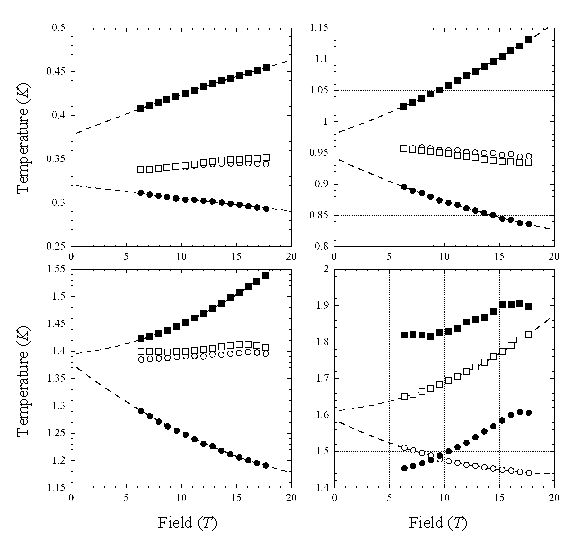
\includegraphics[scale=0.9]{Chapter-dHvABaFe2P2/Figures/Mass/TemperatureCorrection/TemperatureCorrection}
        \caption{Some example temperature readings (squares) set using the sorbtion pump heater. Also shown are corrections (circles) by interpolating to known values. RuOx thermometer is shown in blue, Cernox stage thermometer is shown in red. Second order polynomial fits to the data are shown as lines extrapolated to zero to get a rough estimate of the zero field temperature value.}
        \label{Fig:Exp:TemperatureCorrection}
    \end{center}
\end{figure}
Readings from both thermometers were taken with field sweeps from zero field up to \unit[18]{T} at steady temperatures \unit[0.30]{K}, \unit[0.53]{K}, \unit[0.64]{K}, \unit[1.06]{K} and \unit[1.34]{K}. By interpolating between this data\footnote{Performed using multiquadric radial basis functions from the Scipy Python library.}, the two thermometers can be correctied to agree within $\sim$\unit[0.01]{K}. This interpolation is however limited to temepratures below approximately \unit[1.45]{K} as is shown in the figure for readings at around \unit[1.6]{K}. In these cases, the less reliable method of extrapolating the readings back to zero field using a second order polynomial fit are used as demonstrated with the solid lines in figure~\ref{Fig:Exp:TemperatureCorrection}. In these cases the temeprature is taken to be the mean of the two extrapolated values with the differences defining the error.


\subsubsection{Attenuation due to torque}

An extra attentuation occurs due solely to the nature of the torque oscillation measurement. The attentuation factor is given by,
\begin{equation}
    A_{\Gamma \textrm{(gen)}} = \frac{1}{F}\frac{dF}{d\theta_\perp}VB
\end{equation}
where $V$ is the sample volume and $\theta_\perp$ is angle from the field direction. This can be simplified for a quasi $2d$ metal to,
\begin{equation}
    A_{\Gamma} = |\sin(\theta)|B
\end{equation}
where $\theta$ is the angle from the cylinder axis (usually in the $c$ direction). This means that at along the cylinder axis there will be no oscillations as $A_{\Gamma} \to 0$.


\subsubsection{Background removal}

Previous standard practice was to remove a background polynomial fitted to the field or inverse field from the raw data before taking the \ac{FFT}. With reference to figure~\ref{Fig:Exp:BackgroundSubtractionComparison}, raw torque data taken over a range of angles\footnote{See section\ref{Sec:ResD:AngleDependentMeasurements} for full details} and a strong $B^2$ component can be observed as a result of the $A_{\Gamma}$ term in the \ac{LK} equation (marked `B' in the left panel). As shown in the centre and right panels, subtracting a second order polynomial fitted to the \textit{inverse} field leaves a large artificial angle-dependant oscillation in $1/B$ in the residual which may be misconstrued as a signal from a low frequency Fermi surface orbit, especially since there is an apparent angle dependence -- no such peak is seen for the flat curves at `A' and `C'. For this reason it is recommended to subtract a second order polynomial fitted to field rather than inverse field for torque measurements.
\begin{figure}[h!]
    \begin{center}
        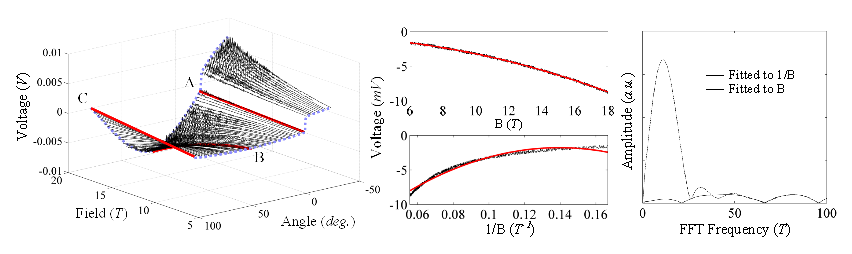
\includegraphics[scale=0.9]{Chapter-ExperimentalTechnique/Figures/ComparisonBackgroundSubtraction/ComparisonBackgroundSubtraction}
        \caption{Left panel shows the angle dependance of the raw torque signal  clearly showing a negative $B^2$ background for $\theta>0$ and a positive $B^2$ background for $\theta<0$. Centre panels show a simulated $B^2$ background with $\sim\unit[0.5]{mV}$ of noise, similar in scale to that of `B' in the first panel, fitted to a 2nd order polynomial with field on top and inverse field on the bottom. The right panel shows the resulting \ac{FFT}s.}
        \label{Fig:Exp:BackgroundSubtraction}
    \end{center}
\end{figure}

\subsection{Measuring the spin mass}

\TODO{Need to do investigation first}

\subsection{Extracting effective mass from the temperature dependence}
\label{Sec:Exp:ExtractingEffMassTemperatureDependence}

Of all the damping terms in the \ac{LK} equation, only $A_T$ (eqn.~\ref{Eqn:Theo:TemperatureTerm}) has any kind of temperature dependancy. This term also features the effective mass. By measuring oscillations at a fixed angle but with varying temperatures, the effective mass can be determined in a number of ways.

\subsubsection{Basic \ac{LK} formula fitting}

The simplest technique to extract the effective mass is to extract the amplitude of the oscillations from \acp{FFT} of the data at various $T$ and then perform a least squares fit to eqn.~\ref{Eqn:Theo:TemperatureTerm}. A particular problem with this approach is that it is not clear what value of $B$ should be used since the \acp{FFT} cover a range of fields. Generally the simplest thing to do is to take the \acp{FFT} over a small a range as possible and then take the field to be equal to the averaged inverse field\footnote{That is $B_{\textrm{av.}}^{-1} = \frac{1}{2}(B_{\textrm{min}}^{-1} + B_{\textrm{max}}^{-1})$}. 

There are two problems with this approach. First the amplitude tends to decreases with narrowing field range meaning weak oscillations may require larger field intervals. Secondly wider field ranges mean other attenuation factors --- which are also functions of $B$ --- affect the amplitude across the field sweep. The primary problem in this case is the Dingle term which has an exponential dependence on $B$.

Nonetheless, simple \ac{LK} fits are usually the first port of call and serve as a first approximation to the final result. For this investigation though, since we found some disagreement within the data, we employed a couple of additional techniques described below to overcome this shortcoming.

\subsubsection{Retrofitting ansatz \ac{LK} formulae}
\label{Sec:Exp:LKRetrofitting}

One of the primary field-dependant contributions to the oscillation amplitude is the Dingle term scattering (equation \ref{Eqn:Theo:DingleTerm}) which has an exponential dependence with temperature. The Dingle factor, $\alpha = -\pi p m_0/e\tau$, can be determined by fitting a simplified version of equation \ac{LK} equation,
\begin{equation}
    \Gamma_{\textrm{sim}} =  A_D(\alpha, B) \sqrt{B} \sin{\left(\frac{2\pi F}{B} + \phi \right)}
\end{equation}
 to oscillations which have been band pass filtered to reduce the number of contributions from other extremal orbits and hence the number of necessary fitting parameters. Once we have the Dingle term and also the peak frequency for a particular orbit, simulated oscillations are generated using the same equation but including the temperature term, $A_T(m^*_{\textrm{therm}}, B)$, for a range of ansatz effective thermal masses. We then fit this to the \ac{LK} equation as described in the previous section. The mass that results from the fit is different from the actual effective mass used as the \ac{LK} fit has been affected by the Dingle term contribution. When we find a simulated oscillation that outputs the same effective thermal mass as the plain \ac{LK} fit on the actual data we then take the ansatz thermal mass for that matching fit to be the corrected thermal mass.

The filtering used to originally separate out the frequencies is band pass \ac{FFT} using a Hann window.  This is adjusted in size and roll off width according to the peak. Occasionally, the peaks are too close together to effectively filter out individually and so two or three peaks were fitted at a time using a linear combination of the simplified equation above.

The initial fits were filtered using a Delphi program written by Prof. Carrington and fits to find $\alpha$ were performed in Kaleidagraph. Ansatz fits were found using a binary search technique using a Python script.


\subsubsection{`Microfitting' the \ac{LK} formula}
\label{Sec:Exp:LKMicrofitting}

A second technique is to filter out the individual orbit frequency by again using an \ac{FFT} filter and a Hann window, and this time fitting small sections of sine curve ($\sim 1.5$--$3$ wavelengths) directly to the filtered torque data. This gives a field dependent value for the amplitude which can then be fitted to the standard $A_T$ form for many values of $B$. The result is a plot of mass values against $B$. Theoretically, these should plateau to give a constant value for the effective thermal mass.

Calculations were performed using a Python script to filter the data, perform the `microfits' and then perform the \ac{LK} fits. The script was tested using simulated data.


